\documentclass[12pt]{article}
\usepackage{amsmath,amsfonts,times}
\usepackage{graphicx,color,tikz,pgfplots}
\usepackage[paperwidth=10.1cm,paperheight=8.1cm,lmargin=0in,rmargin=0in,tmargin=0.in,bmargin=0.in]{geometry}
\usepackage{bm}
\usetikzlibrary{arrows,shadings,shapes.arrows,decorations.pathreplacing,calc, positioning}
\usepgfplotslibrary{fillbetween}

\begin{document}
\centering
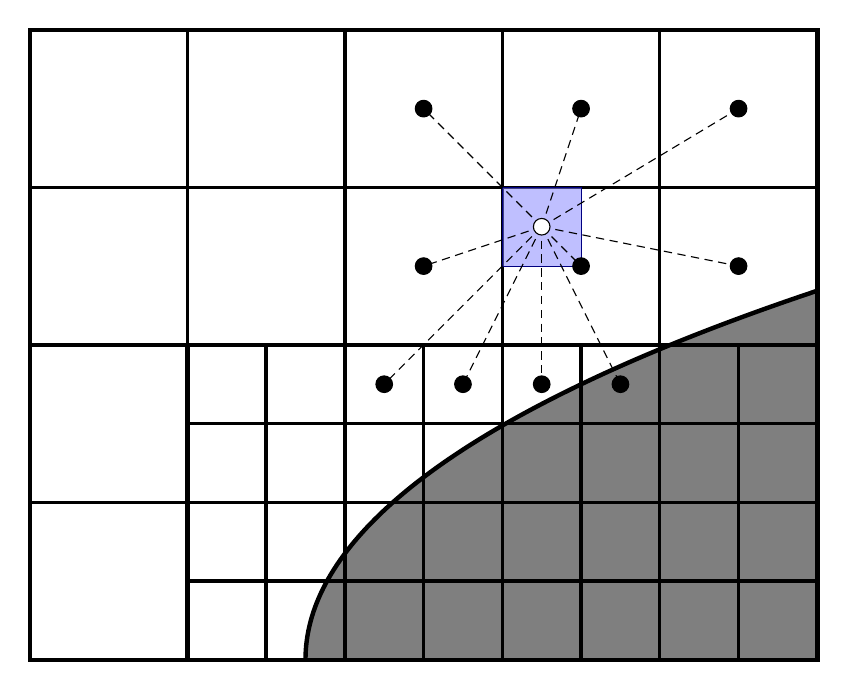
\begin{tikzpicture}[on grid]

  % Parent grid
  \draw[step=20mm, black, very thick] (0,0) grid  (10,8); %defining grids
  \draw[black,ultra thick] (0,0) rectangle (10,8); %marking borders

  % Refined grid
  \draw[step=10mm, black, very thick] (2,0) grid  (10,4); %defining grids
  \draw[black,ultra thick] (2,0) rectangle (10,4);%marking borders

  % Ghost region
  \draw[draw=blue!50!black, fill=blue!50!white, fill opacity=0.5] (6,5) rectangle (7,6); %defining grids  

  % Stencil region for cut-cell
  %% \draw[red!50!black, densely dashed, fill=red!50!white, thin] (5,3) grid (6,4); 
  %% \draw[red!50!black, fill=blue!50!white, thick, fill opacity=0.2] (4,2) rectangle (8,6); %marking borders
  %% \draw[red!50!black, fill=red!50!white, thick, fill opacity=1.0] (6,3) rectangle (7,4); %marking borders

  % Interpolation stencil
  \draw[densely dashed] (6.5,5.5) -- (7,5);
  \draw[densely dashed] (6.5,5.5) -- (9,5);
  \draw[densely dashed] (6.5,5.5) -- (9,7);
  \draw[densely dashed] (6.5,5.5) -- (7,7);
  \draw[densely dashed] (6.5,5.5) -- (5,7);
  \draw[densely dashed] (6.5,5.5) -- (5,5);
  \draw[densely dashed] (6.5,5.5) -- (4.5,3.5);
  \draw[densely dashed] (6.5,5.5) -- (5.5,3.5);
  \draw[densely dashed] (6.5,5.5) -- (6.5,3.5);
  \draw[densely dashed] (6.5,5.5) -- (7.5,3.5);
  
  \draw[black,fill=white] (6.5,5.5) circle (3pt);
  \draw[black,fill=black] (4.5,3.5) circle (3pt);
  \draw[black,fill=black] (5.5,3.5) circle (3pt);
  \draw[black,fill=black] (6.5,3.5) circle (3pt);
  \draw[black,fill=black] (7.5,3.5) circle (3pt);
  \draw[black,fill=black] (5,5) circle (3pt);
  \draw[black,fill=black] (5,7) circle (3pt);
  \draw[black,fill=black] (7,5) circle (3pt);
  \draw[black,fill=black] (7,7) circle (3pt);
  \draw[black,fill=black] (9,5) circle (3pt);
  \draw[black,fill=black] (9,7) circle (3pt);



  %% \draw[black,fill=black] (5.5,2.5) circle (3pt);
    
  %% \draw[black,fill=black] (4.5,3.5) circle (3pt);
  %% \draw[black,fill=black] (5.5,3.5) circle (3pt);
  %% \draw[black,fill=black] (6.5,3.5) circle (3pt);
  %% \draw[black,fill=black] (7.5,3.5) circle (3pt);

  %% \draw[black,fill=black] (4.5,4.5) circle (3pt);
  %% \draw[black,fill=black] (5.5,4.5) circle (3pt);
  %% \draw[black,fill=black] (6.5,4.5) circle (3pt);
  %% \draw[black,fill=black] (7.5,4.5) circle (3pt);

  %% \draw[black,fill=black] (4.5,5.5) circle (3pt);
  %% \draw[black,fill=black] (5.5,5.5) circle (3pt);
  %% \draw[black,fill=black] (6.5,5.5) circle (3pt);
  %% \draw[black,fill=black] (7.5,5.5) circle (3pt);


  %EB
  \clip(0,0) rectangle (10,8);  
  \draw[black, ultra thick, draw=black, fill=black, fill opacity=0.5] (53.5,0.0) ellipse (50cm and 9.5cm);



\end{tikzpicture}

\end{document} 
